\chapter{Introduction}
\label{chap:introduction}
\setcounter{page}{1}
\pagenumbering{arabic}

In recent years, computer vision has made great progress. People have achieved good results in some simple tasks and have been applied in many fields, such as image classification~\cite{yu2017convolutional, lu2007survey}, image segmentation ~\cite{pham2000current} and face recognition~\cite{ahonen2006face, phillips1996feret}. Now people are no longer satisfied with these basic tasks, but hope that computers can interpret pictures like humans to obtain more information, such as the attributes of objects,  the motion of objects, and the relationships between objects, etc. Thus people began to study some complex tasks such as Image Captioning ~\cite{hossain2019comprehensive},  Visual Question Answer~\cite{antol2015vqa}, and  visual relationship detection (VRD). 

\begin{figure}[!htbp]
	\centering
	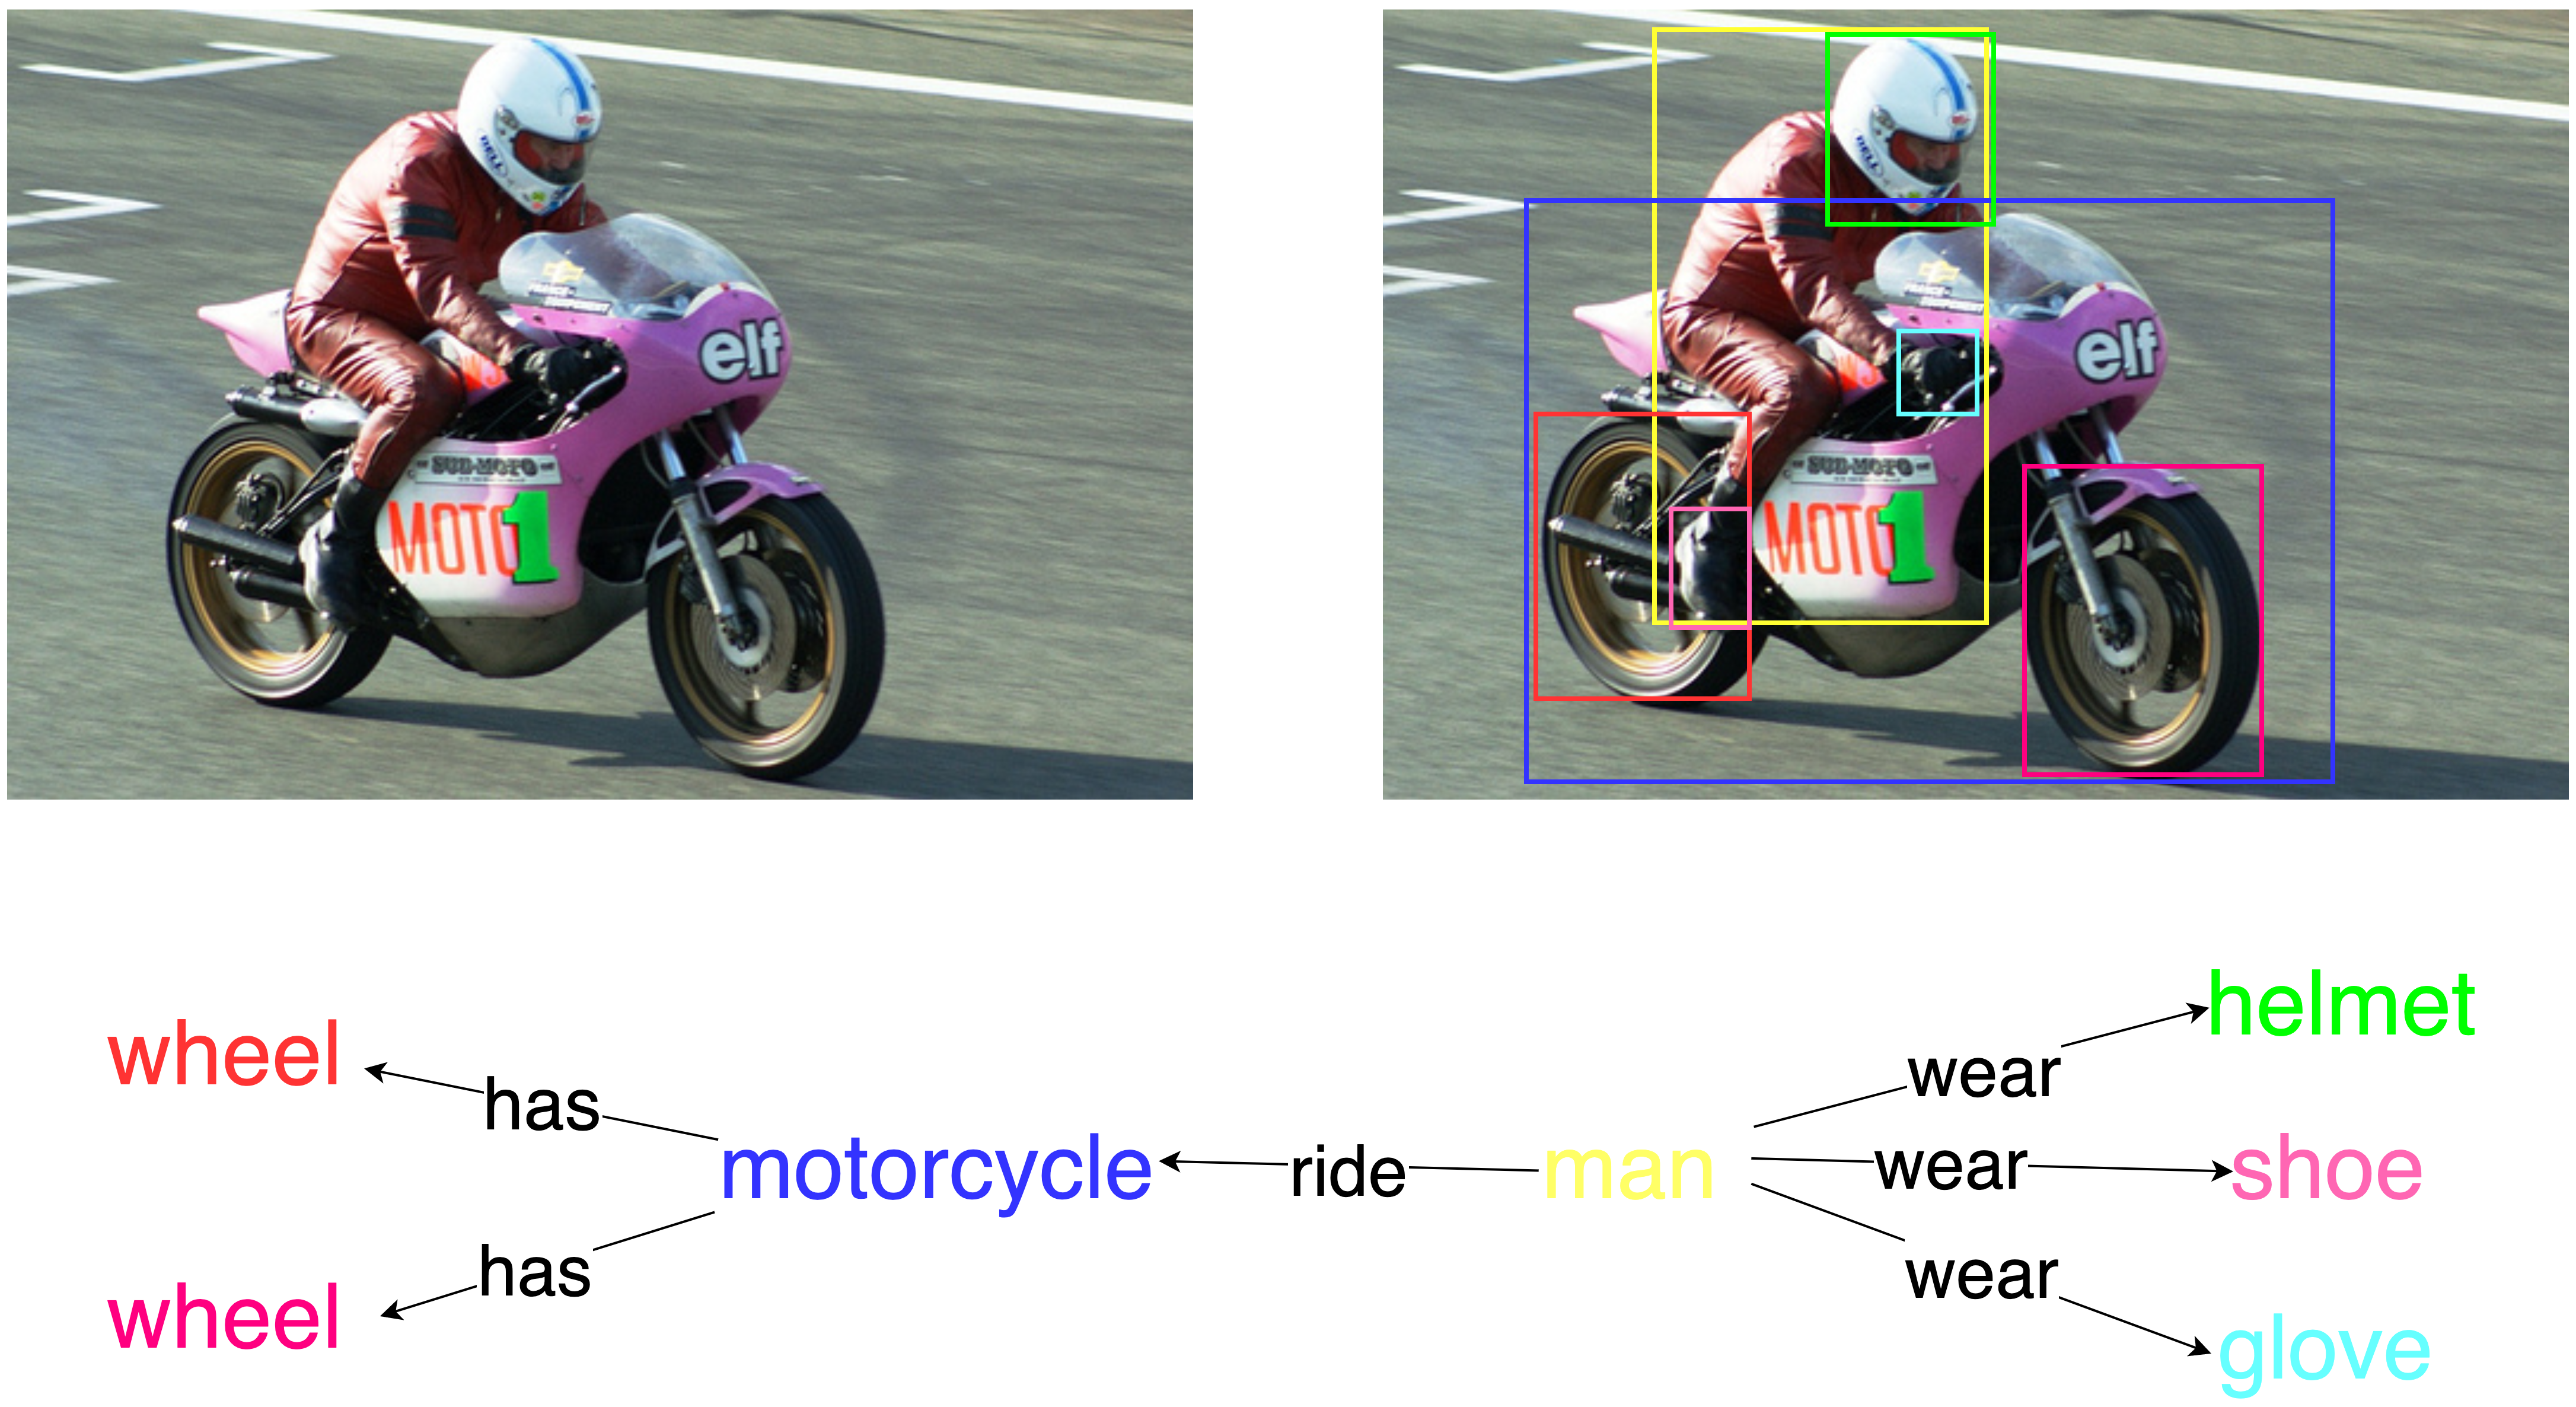
\includegraphics[width = 0.9 \textwidth]{figures/senen_graph.png}
	\caption[A example of visual relationship detection]
	{ A example of visual relationship detection: The upper left corner is the original input image, the upper right corner is the result of object detection, and the lower one is the relationship detection}
	\label{fig:sene}
\end{figure}

The visual relationship detection task not only needs to recognize the objects in the image and their positions, but also recognize the relationship between the objects, that is, the connection between the target objects, which can be expressed as a triplet-Relationship: $\left \langle subject, predicate, object\right \rangle$. For example, in figure~\ref{fig:sene}, a VRD task includes identifying instances in the image: motorcycle, man, helmet, wheels, etc., as well as identifying the relationship between them, like $\left \langle man, ride, motorcycle\right \rangle$, $\left \langle man, wear, helmet\right \rangle$, $\left \langle motor, has, wheel\right \rangle$, etc..


\section{Motivation}

Visual relationship detection connects objects in images with predicates, and also connects low-level vision and high-level language (see Figure ~\ref{fig:vrd}). This means that visual relationship detection can provide high-level tasks, such as image captioning~\cite{hossain2019comprehensive} for easier-to-understand information; it can also improve low-level tasks such as object detection using scene context. Visual relationship detection is an essential step to realize that computers can understand images as intelligently as humans.

\begin{figure}[!htbp]
	\centering
	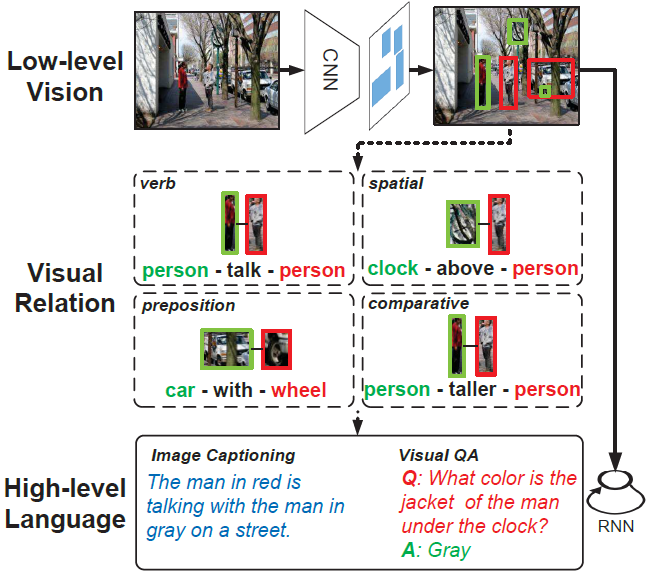
\includegraphics[width = 0.7 \textwidth]{figures/VRD.png}
	\caption[Connection between low-level vision and high-level vision]
	{ Visual relationship detection understands object interactions directly, which offer further semantic information for applications such as image captioning and QA. Figure obtained from ~\cite{zhang2017visual}}
	\label{fig:vrd}
\end{figure}

In recent years, with the proposal of the Transformer structure~\cite{vaswani2017attention}(see in section~\ref{section:transformer}), people have found that it not only achieves excellent performance in natural language processing tasks, but also has a very wide range of applications in computer vision, such as the DETR model~\cite{carion2020end} (see Figure ~\ref{fig:detr})proposed by Nicolas et al., using the Encoder-Decoder structure of the Transformer, The object detection effect of DETR is not inferior to Faster R-CNN~\cite{ren2016faster}. Thus we want to study the possibility of transformer structure in VRD problem.


There are three main related tasks of visual relationship detection problem: Predicate classification(PredCLS), which only needs to predict the relationship. Scene graph classification(SGCLS) needs to classify objects and  predict relationships. Scene graph detection(SGDET) needs to not only classify objects and  predict relationship, but also locate  the relationship.

In this thesis we utilise transformer encoder-decoder structure, aiming solving problems regarding to Visual Relation Detection(VRD), meanwhile, we also focus the use of attention mechanism to define the VRD problems, which the researchers should pay more attention to.

The motivaton for our task are mainly summarized as follows:

\begin{enumerate}[\qquad 1.]
	\item Given object detection has been properly solved by detr, in which transformer structure considered as basic foundation for detr. Therefore, we tend to find solution for relation detection through transformer structure as well.
	\item In order to detect objects, the transformer structure extracts object features with the implements of learnable query. we don't expect learnable query has any physical meanings . but in SGCLS and PredCLS, which are submission for VRD. the complete object detection is unnecessary. because they are known as condition for the task. but learnable query doesn't cover this information, so learnable query isn't able to coping with these tasks. Thus, we need to develop a query, that indicates all the known information of object, and obtain corresponding object feature.
	\item As we use transformer structure, it is important that we never overlook the attention mechanism. we need to understand the operation of  attention in the task of vrd. for example, by studying the attention between subject and object, we can decide, if there is a relation between them. or by studying the attention between relation and object, we will learn, which objects the relation pay most attention to. all the mentioned steps can help us understand the role of each object and how objects are related and influenced bz others in the context of the whole image.
	\item The most important challenge is to predict the correct predicate, that describe the relation between two objects. To realise our goals, we designed a relation decoder, which helps to exploit semantic and spatial co-relation among various objects.
\end{enumerate}
 

\section{Contribution}

In this thesis, we provide  an efficient framework based on Encoder-Decoder of the  Transformer structure  for visual relationship detection that detects the interactions between objects in the image. The main work and contributions are summarized as following:
\begin{enumerate}[\qquad  1.]
	\item By using the transformer structure, we have solved the vrd problem properly. and completed  each submission outstandingly. our design has proven the feasibility of the transformer in solving the vrd problem.
	\item We propose an object query, which replace the learnable query to maintain consistency with each object, and expresses the visual information of the object through the transformer.
	\item We have designed the relation decoder and established a new context propagation across relationships and objects, which greatly improved the results of our tasks.
\end{enumerate}


\section{Organization of the Thesis}
This thesis is structured as follows:

In Chapter~\ref{chap:relatedwork} , we will discuss about the related works. Some advanced researches and models about object detection and visual relationship detection are introduced briefly. We also demonstrate their contributions and limitations.

In Chapter ~\ref{chap:bg}, the theories about Transformer and other important models and algorithm such as Faster R-CNN , Hungarian matching and ranking loss  will be introduced.

In Chapter ~\ref{chap:framework}, the proposed framework will be shown in detail.

In Chapter ~\ref{chap:experiment}, the experimental results will be presented and analyzed in detail. Our proposed framework are evaluated on Visual Genome with three standard evaluation metrics.

In Chapter ~\ref{chap:conclusion}, we conclude our work finally and point out the future research direction.